\documentclass[11pt]{article}

\usepackage[utf8]{inputenc}
\usepackage[T1]{fontenc}
\usepackage{lmodern}
\usepackage{amsmath, amssymb}
\usepackage{xcolor}
\usepackage{tcolorbox}
\usepackage{graphicx}
\graphicspath{{images/}}
\usepackage{tikz}
\usepackage{float}
\usepackage{hyperref}
\usepackage{enumitem}
\usepackage{caption}
\usepackage{listings}
\usepackage[margin=1in]{geometry}

\usetikzlibrary{shapes, arrows.meta, positioning, decorations.pathreplacing}

\hypersetup{
  colorlinks=true,
  linkcolor=blue,
  urlcolor=blue,
  citecolor=blue
}


% --- Semantic tcolorbox styles ---
\definecolor{defblue}{RGB}{41, 98, 163}
\definecolor{insightgreen}{RGB}{46, 139, 87}
\definecolor{warnorange}{RGB}{204, 119, 34}
\definecolor{recapgray}{RGB}{100, 100, 100}
\definecolor{actionviolet}{RGB}{106, 61, 154}
\definecolor{resultteal}{RGB}{0, 128, 128}

\newtcolorbox{defbox}[1][]{colback=defblue!5!white, colframe=defblue!80, fonttitle=\bfseries, #1}
\newtcolorbox{insightbox}[1][]{colback=insightgreen!5!white, colframe=insightgreen!80, fonttitle=\bfseries, #1}
\newtcolorbox{warnbox}[1][]{colback=warnorange!6!white, colframe=warnorange!80, fonttitle=\bfseries, #1}
\newtcolorbox{recapbox}[1][]{colback=recapgray!6!white, colframe=recapgray!70, fonttitle=\bfseries, #1}
\newtcolorbox{actionbox}[1][]{colback=actionviolet!5!white, colframe=actionviolet!70, fonttitle=\bfseries, #1}
\newtcolorbox{resultbox}[1][]{colback=resultteal!5!white, colframe=resultteal!80, fonttitle=\bfseries, #1}


% --- TikZ diagram colors ---
\definecolor{inputblue}{RGB}{41, 98, 163}
\definecolor{neuronorange}{RGB}{230, 140, 30}
\definecolor{activgreen}{RGB}{46, 139, 87}
\definecolor{outputviolet}{RGB}{106, 61, 154}
\definecolor{arrowgray}{RGB}{80, 80, 80}
\definecolor{layer1color}{RGB}{41, 98, 163}
\definecolor{layer2color}{RGB}{204, 119, 34}
\definecolor{layer3color}{RGB}{46, 139, 87}
\definecolor{outputlayercolor}{RGB}{0, 128, 128}


% --- Code listing style ---
\definecolor{codebg}{RGB}{248, 248, 248}
\definecolor{codeframe}{RGB}{200, 200, 200}
\definecolor{codekw}{RGB}{41, 98, 163}
\definecolor{codecomment}{RGB}{100, 140, 100}
\definecolor{codestring}{RGB}{163, 61, 61}

\lstdefinestyle{pythonstyle}{
  language=Python,
  backgroundcolor=\color{codebg},
  frame=single,
  rulecolor=\color{codeframe},
  basicstyle=\ttfamily\small,
  keywordstyle=\color{codekw}\bfseries,
  commentstyle=\color{codecomment}\itshape,
  stringstyle=\color{codestring},
  numbers=left,
  numberstyle=\tiny\color{gray},
  numbersep=8pt,
  showstringspaces=false,
  breaklines=true,
  tabsize=4,
  xleftmargin=1.5em,
  framexleftmargin=1.5em,
  aboveskip=1em,
  belowskip=1em,
  morekeywords={True, False, None, self, np, plt},
}

\lstset{style=pythonstyle}


\begin{document}

\begin{titlepage}
    \centering
    \vspace*{2.2cm}

    {\Large \textbf{DEEP LEARNING FROM SCRATCH}}\\[0.4em]
    A Guide for Self-Learners\\[2.5em]

    {\Huge \bfseries Episode VII}\\[0.4em]
    {\LARGE \textit{Horizon of Depth}}\\[2em]

    \vspace{0.8cm}

    {\large\itshape
    Two layers was the beginning.\\
    Now we remove the limit.\\[0.8em]
    {\Large \textbf{Now we cross the horizon.}}
    }

    \vspace{0.8cm}

    \begin{tcolorbox}[colback=black!3!white, colframe=black!20!white, width=0.8\textwidth, sharp corners, boxrule=0.4pt]
    \centering
    \itshape

    {\Large One list. Any architecture. Infinite depth.}\\[1em]

    \textbf{Why this episode?}\\[0.3em]
    Your 2-layer network works. But it's hardcoded.\\
    What if you wanted 5 layers? Or 50?\\
    In this episode, you'll generalize everything ---\\
    and discover that the code barely changes.
    \end{tcolorbox}

    \vspace{1.5cm}

    \begin{center}
    \itshape
        {\Large \textit{``Simplicity is the ultimate sophistication.''}}\\
        \vspace{0.2em}
        {\large -- Leonardo da Vinci}
    \end{center}

    \vfill

    {\large \textbf{Pierre Chambet}}\\[0.3em]
    {\small March 2026}\\[1em]
    \rule{0.8\textwidth}{0.4pt}\\[0.4em]
    {\small Part of the \textit{Deep Learning From Scratch} series --- an independent reconstruction of AI.}

\end{titlepage}

\tableofcontents

\vspace{1.5em}

\begin{defbox}[title=What You'll Learn in This Episode]
After these pages, you'll be able to build a neural network of \textbf{any depth} --- not just 2 layers, but $L$ layers --- from scratch.

\begin{enumerate}[label=\textbf{\arabic*.}]
  \item How a single \textbf{dimensions list} defines an entire architecture
  \item How to \textbf{generalize initialization} with a loop
  \item How to write \textbf{forward propagation} for $L$ layers
  \item How to derive and implement \textbf{generalized backpropagation}
  \item How to test your network on \textbf{increasingly complex datasets}
  \item Why \textbf{deeper networks} don't always mean better results
  \item Where the next frontier lies: \textbf{discipline over power}
\end{enumerate}
\end{defbox}

\newpage

%% ============================================================
%% SECTION 1 --- INTRODUCTION
%% ============================================================
\section{What If?}

In Episode VI, you built a neural network from scratch.

It worked. It classified toxic plants with near-perfect accuracy. It even handled real images --- cats and dogs --- with respectable results.

But here's the thing: that network was \textbf{hardcoded}.

Two layers. Exactly two. The initialization function created \texttt{W1}, \texttt{b1}, \texttt{W2}, \texttt{b2} --- four parameters, by name, one by one. The forward propagation computed \texttt{Z1}, \texttt{A1}, \texttt{Z2}, \texttt{A2} --- again, hardcoded. The backpropagation derived \texttt{dW1}, \texttt{db1}, \texttt{dW2}, \texttt{db2} --- six lines, each written by hand.

What if you wanted three layers?

You'd have to rewrite the initialization. Rewrite forward propagation. Rewrite backpropagation. Add more variables. More lines. More chances for bugs.

What about five layers? Ten?

\textit{That approach doesn't scale.}

\begin{insightbox}[title=The Core Idea]
The operations at each layer are \textbf{identical}: multiply, add bias, activate. The only things that change are the dimensions.

If the operations are the same, we can use a \textbf{loop}.

And if we use a loop, we can handle \textbf{any number of layers}.
\end{insightbox}

That's what this episode is about. We're going to take every function from Episode VI and replace the hardcoded indices with a loop. The result: a neural network of \textbf{any depth}, controlled by a single list.

\begin{actionbox}[title=Let's Build]
Open the companion notebook. Every function we discuss here is ready to run.

\textbf{Colab:} \url{https://colab.research.google.com/github/Pchambet/Deep-Learning-from-Scratch/blob/main/notebooks/07_horizon_of_depth.ipynb}
\end{actionbox}

\begin{recapbox}[title=Where We Left Off]
Episode VI gave you 7 working functions:
\begin{itemize}
  \item \texttt{initialisation(n0, n1, n2)} --- hardcoded for 2 layers
  \item \texttt{forward\_propagation(X, parameters)} --- Z1, A1, Z2, A2
  \item \texttt{back\_propagation(y, parameters, activations)} --- 6 gradients
  \item \texttt{update(gradients, parameters, learning\_rate)}
  \item \texttt{predict(X, parameters)}
  \item \texttt{neural\_network(...)} --- the training loop
  \item \texttt{decision\_boundary(...)} --- visualization
\end{itemize}
Today, we generalize all of them to $L$ layers.
\end{recapbox}


%% ============================================================
%% SECTION 2 --- THE ARCHITECTURE LIST
%% ============================================================
\section{The Architecture List}

In Episode VI, the architecture was defined by three numbers: \texttt{n0} (input dimension), \texttt{n1} (hidden neurons), and \texttt{n2} (output). You passed them as separate arguments.

Now, we replace them with a single list:

\begin{lstlisting}
dimensions = [2, 32, 32, 1]
\end{lstlisting}

This single line says:
\begin{itemize}
  \item \textbf{Input layer}: 2 features
  \item \textbf{Hidden layer 1}: 32 neurons
  \item \textbf{Hidden layer 2}: 32 neurons
  \item \textbf{Output layer}: 1 neuron (binary classification)
\end{itemize}

The number of layers is:
$$L = \texttt{len(dimensions)} - 1$$

For our example: $L = 4 - 1 = 3$ layers (two hidden + one output).

\begin{defbox}[title=The Dimensions List]
A neural network architecture is fully defined by:
$$\texttt{dimensions} = [n_0, \; n_1, \; n_2, \; \dots, \; n_L]$$
where $n_0$ is the input dimension, $n_l$ is the number of neurons in layer $l$, and $n_L$ is the output dimension.

\textbf{One list. Any architecture. Any depth.}
\end{defbox}

Want a deeper network? Just add numbers:

\begin{lstlisting}
dimensions = [4096, 64, 32, 16, 1]  # 4 layers
dimensions = [4096, 128, 128, 64, 32, 16, 1]  # 6 layers
\end{lstlisting}

No code changes. Just a longer list.

\begin{figure}[H]
    \centering
    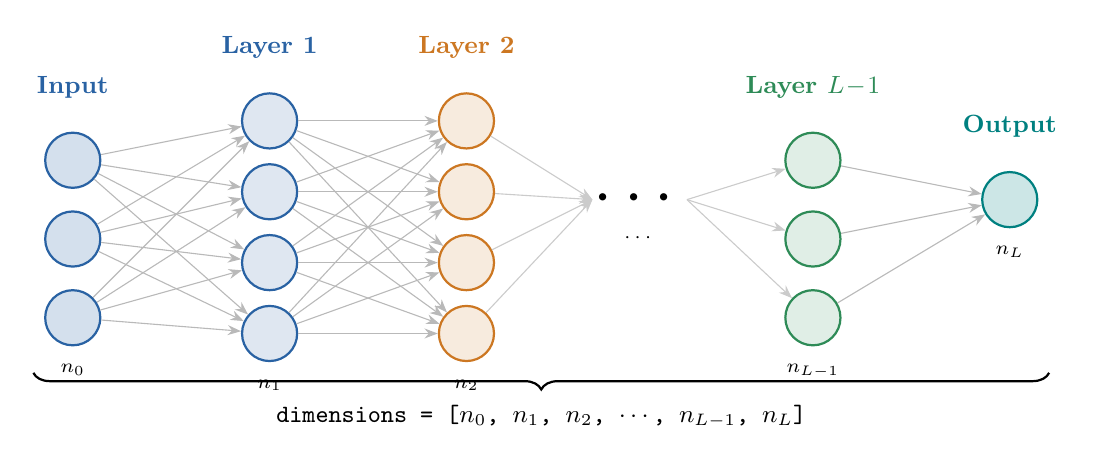
\begin{tikzpicture}[
        node distance=2.2cm,
        neuron/.style={circle, draw, minimum size=0.7cm, line width=0.8pt},
        >=Stealth
    ]
    % Input layer
    \foreach \i in {1,2,3} {
        \node[neuron, fill=inputblue!20, draw=inputblue] (i\i) at (0, -\i*1.0 + 0.5) {};
    }
    \node[above=0.3cm of i1, font=\small\bfseries, text=inputblue] {Input};
    \node[below=0.1cm of i3, font=\scriptsize] {$n_0$};

    % Hidden layer 1
    \foreach \i in {1,2,3,4} {
        \node[neuron, fill=layer1color!15, draw=layer1color] (h1\i) at (2.5, -\i*0.9 + 0.9) {};
    }
    \node[above=0.3cm of h11, font=\small\bfseries, text=layer1color] {Layer 1};
    \node[below=0.1cm of h14, font=\scriptsize] {$n_1$};

    % Hidden layer 2
    \foreach \i in {1,2,3,4} {
        \node[neuron, fill=layer2color!15, draw=layer2color] (h2\i) at (5.0, -\i*0.9 + 0.9) {};
    }
    \node[above=0.3cm of h21, font=\small\bfseries, text=layer2color] {Layer 2};
    \node[below=0.1cm of h24, font=\scriptsize] {$n_2$};

    % Dots
    \node[font=\Huge] at (7.2, -1.0) {$\cdots$};
    \node[below=0.3cm, font=\scriptsize] at (7.2, -1.0) {$\cdots$};

    % Hidden layer L-1
    \foreach \i in {1,2,3} {
        \node[neuron, fill=layer3color!15, draw=layer3color] (hL\i) at (9.4, -\i*1.0 + 0.5) {};
    }
    \node[above=0.3cm of hL1, font=\small\bfseries, text=layer3color] {Layer $L\!-\!1$};
    \node[below=0.1cm of hL3, font=\scriptsize] {$n_{L-1}$};

    % Output layer
    \node[neuron, fill=outputlayercolor!20, draw=outputlayercolor] (o1) at (11.9, -1.0) {};
    \node[above=0.3cm of o1, font=\small\bfseries, text=outputlayercolor] {Output};
    \node[below=0.1cm of o1, font=\scriptsize] {$n_L$};

    % Arrows: input to hidden 1
    \foreach \i in {1,2,3} {
        \foreach \j in {1,2,3,4} {
            \draw[->, arrowgray!40] (i\i) -- (h1\j);
        }
    }
    % Arrows: hidden 1 to hidden 2
    \foreach \i in {1,2,3,4} {
        \foreach \j in {1,2,3,4} {
            \draw[->, arrowgray!40] (h1\i) -- (h2\j);
        }
    }
    % Arrows: hidden 2 to dots (symbolic)
    \foreach \i in {1,2,3,4} {
        \draw[->, arrowgray!30] (h2\i) -- (6.6, -1.0);
    }
    % Arrows: dots to layer L-1
    \foreach \i in {1,2,3} {
        \draw[->, arrowgray!30] (7.8, -1.0) -- (hL\i);
    }
    % Arrows: layer L-1 to output
    \foreach \i in {1,2,3} {
        \draw[->, arrowgray!40] (hL\i) -- (o1);
    }

    % Brace for dimensions
    \draw[decorate, decoration={brace, amplitude=6pt, mirror}, thick]
        (-0.5, -3.2) -- (12.4, -3.2) node[midway, below=8pt, font=\small] {
            \texttt{dimensions = [$n_0$, $n_1$, $n_2$, $\cdots$, $n_{L-1}$, $n_L$]}
        };
    \end{tikzpicture}
    \caption{A generic $L$-layer neural network. The entire architecture is defined by the \texttt{dimensions} list.}
\end{figure}


%% ============================================================
%% SECTION 3 --- INITIALIZATION
%% ============================================================
\section{Initialization --- The Loop}

Let's start with the comparison. Here's what initialization looked like in Episode VI:

\begin{lstlisting}[title={\small Episode VI --- Hardcoded for 2 layers}]
def initialisation(n0, n1, n2):
    parameters = {
        'W1': np.random.randn(n1, n0),
        'b1': np.random.randn(n1, 1),
        'W2': np.random.randn(n2, n1),
        'b2': np.random.randn(n2, 1),
    }
    return parameters
\end{lstlisting}

Four lines, four parameters, two layers. Hardcoded.

Now here's the generalized version:

\begin{lstlisting}[title={\small Episode VII --- Any number of layers}]
def initialisation(dimensions):
    parameters = {}
    L = len(dimensions)
    for l in range(1, L):
        parameters[f'W{l}'] = np.random.randn(dimensions[l],
                                               dimensions[l-1])
        parameters[f'b{l}'] = np.random.randn(dimensions[l], 1)
    return parameters
\end{lstlisting}

That's it. The loop creates \texttt{W1}, \texttt{b1}, \texttt{W2}, \texttt{b2}, \ldots, \texttt{WL}, \texttt{bL} --- however many layers you specify.

\begin{insightbox}[title={Same Logic, Different Scale}]
If you call \texttt{initialisation([2, 32, 32, 1])}, the loop creates:
\begin{itemize}
  \item $l=1$: \texttt{W1} shape $(32, 2)$, \texttt{b1} shape $(32, 1)$
  \item $l=2$: \texttt{W2} shape $(32, 32)$, \texttt{b2} shape $(32, 1)$
  \item $l=3$: \texttt{W3} shape $(1, 32)$, \texttt{b3} shape $(1, 1)$
\end{itemize}
Exactly what Episode VI had --- plus one extra layer. Same logic. Just a loop.
\end{insightbox}

Let's verify it works:

\begin{lstlisting}
parameters = initialisation([2, 32, 32, 1])
for key, value in parameters.items():
    print(key, value.shape)
\end{lstlisting}

\begin{resultbox}[title=Output]
\begin{verbatim}
W1 (32, 2)
b1 (32, 1)
W2 (32, 32)
b2 (32, 1)
W3 (1, 32)
b3 (1, 1)
\end{verbatim}
\end{resultbox}

Six parameters instead of four. Three layers instead of two. \textbf{Same function}.


%% ============================================================
%% SECTION 4 --- FORWARD PROPAGATION
%% ============================================================
\section{Forward Propagation --- The Generic Loop}

In Episode VI, forward propagation was four lines:

\begin{lstlisting}[title={\small Episode VI --- Hardcoded}]
Z1 = W1 @ X + b1     # A1 = sigma(Z1)
A1 = 1 / (1 + np.exp(-Z1))
Z2 = W2 @ A1 + b2    # A2 = sigma(Z2)
A2 = 1 / (1 + np.exp(-Z2))
\end{lstlisting}

Look at the pattern: for each layer, we compute $Z = W \cdot A_{\text{prev}} + b$ and then $A = \sigma(Z)$.

The generalized version replaces this with a loop:

\begin{lstlisting}[title={\small Episode VII --- Any depth}]
def forward_propagation(X, parameters):
    activations = {'A0': X}
    L = len(parameters) // 2
    A = X
    for l in range(1, L + 1):
        Z = parameters[f'W{l}'] @ A + parameters[f'b{l}']
        A = 1 / (1 + np.exp(-Z))
        activations[f'A{l}'] = A
    return activations
\end{lstlisting}

Let's break it down:

\begin{enumerate}
  \item We set the input $X$ as the ``zeroth activation'': $A_0 = X$.
  \item For each layer $l$ from $1$ to $L$:
  \begin{itemize}
    \item Compute the pre-activation: $Z_l = W_l \cdot A_{l-1} + b_l$
    \item Apply the sigmoid: $A_l = \sigma(Z_l) = \dfrac{1}{1 + e^{-Z_l}}$
    \item Store $A_l$ in the activations dictionary
  \end{itemize}
  \item Return all activations (we'll need them for backpropagation).
\end{enumerate}

\begin{defbox}[title=Forward Propagation --- General Form]
For a network with $L$ layers:
\begin{align}
A_0 &= X \\
Z_l &= W_l \cdot A_{l-1} + b_l \quad \text{for } l = 1, \dots, L \\
A_l &= \sigma(Z_l) \quad \text{for } l = 1, \dots, L
\end{align}
The output prediction is $\hat{y} = A_L$.

Two operations per layer. $L$ times. That's it.
\end{defbox}

Note the key insight: we store \textbf{all} activations $A_0, A_1, \ldots, A_L$ in a dictionary. We'll need every single one of them during backpropagation --- because each gradient depends on the activation of the previous layer.


%% ============================================================
%% SECTION 5 --- BACKPROPAGATION
%% ============================================================
\section{Generalized Backpropagation}

This is the heart of the episode.

In Episode VI, backpropagation was six specific lines --- each gradient written out explicitly for layers 1 and 2. Now we need to generalize it to \textbf{any number of layers}.

The good news: the math doesn't change. The chain rule still works the same way. We just apply it $L$ times instead of twice.

\subsection{The Equations}

\begin{defbox}[title=Generalized Backpropagation Equations]
For the \textbf{output layer} ($l = L$):
$$dZ_L = A_L - y$$

For any \textbf{hidden layer} ($l = L-1, \; L-2, \; \ldots, \; 1$):
$$dZ_l = \left(W_{l+1}^T \cdot dZ_{l+1}\right) \odot A_l \odot (1 - A_l)$$

For \textbf{every layer} ($l = L, \; L-1, \; \ldots, \; 1$):
\begin{align}
dW_l &= \frac{1}{m} \cdot dZ_l \cdot A_{l-1}^T \\[0.3em]
db_l &= \frac{1}{m} \sum dZ_l
\end{align}
\end{defbox}

Let's make sure you understand what each term means:

\begin{itemize}
  \item $dZ_L = A_L - y$ --- the error at the output. This is \textbf{identical} to Episode VI.
  \item $dZ_l = (W_{l+1}^T \cdot dZ_{l+1}) \odot A_l \odot (1 - A_l)$ --- the error \textbf{propagated backward} from layer $l+1$ to layer $l$. The term $A_l \odot (1 - A_l)$ is the derivative of the sigmoid activation.
  \item $dW_l$ and $db_l$ --- the gradients with respect to the weights and biases at layer $l$. These are computed the same way at every layer.
\end{itemize}

\begin{insightbox}[title=The Pattern]
At each layer, the same three things happen:
\begin{enumerate}
  \item Receive the error from the layer above ($dZ$)
  \item Compute the gradients for this layer ($dW$, $db$)
  \item Pass the error backward to the layer below
\end{enumerate}
This is why it's called \textbf{back}propagation --- the error flows backward through the network.
\end{insightbox}

\subsection{The Code}

\begin{lstlisting}[title={\small Generalized Backpropagation}]
def back_propagation(y, parameters, activations):
    m = y.shape[1]
    L = len(parameters) // 2

    # Output layer error
    dZ = activations[f'A{L}'] - y
    gradients = {}

    # Loop backward through the layers
    for l in reversed(range(1, L + 1)):
        gradients[f'dW{l}'] = 1/m * dZ @ activations[f'A{l-1}'].T
        gradients[f'db{l}'] = 1/m * np.sum(dZ, axis=1, keepdims=True)

        # If not the first layer, propagate error backward
        if l > 1:
            dA_prev = parameters[f'W{l}'].T @ dZ
            A_prev = activations[f'A{l-1}']
            dZ = dA_prev * A_prev * (1 - A_prev)

    return gradients
\end{lstlisting}

Compare this to Episode VI's six hardcoded lines:

\begin{lstlisting}[title={\small Episode VI --- Hardcoded for 2 layers}]
dZ2 = A2 - y
dW2 = 1/m * dZ2 @ A1.T
db2 = 1/m * np.sum(dZ2, axis=1, keepdims=True)
dZ1 = W2.T @ dZ2 * A1 * (1 - A1)
dW1 = 1/m * dZ1 @ X.T
db1 = 1/m * np.sum(dZ1, axis=1, keepdims=True)
\end{lstlisting}

\begin{warnbox}[title=Same Math --- Just a Loop]
The generalized version does \textbf{exactly} the same thing. It starts at the output ($l = L$), computes $dW_L$ and $db_L$, then propagates the error backward to $l = L-1$, and repeats.

If $L = 2$, the loop runs twice --- and produces the exact same six gradients as Episode VI.

If $L = 10$, it runs ten times. \textbf{No code changes.}
\end{warnbox}


%% ============================================================
%% SECTION 6 --- UPDATE AND PREDICT
%% ============================================================
\section{Update and Predict}

These two functions are almost trivially simple.

\subsection{Update --- Gradient Descent for All Layers}

\begin{lstlisting}
def update(gradients, parameters, learning_rate):
    L = len(parameters) // 2
    for l in range(1, L + 1):
        parameters[f'W{l}'] -= learning_rate * gradients[f'dW{l}']
        parameters[f'b{l}'] -= learning_rate * gradients[f'db{l}']
    return parameters
\end{lstlisting}

Same gradient descent rule as before: $W \leftarrow W - \alpha \cdot dW$. Applied to every layer in a loop.

\subsection{Predict --- Identical to Episode VI}

\begin{lstlisting}
def predict(X, parameters):
    activations = forward_propagation(X, parameters)
    L = len(parameters) // 2
    A = activations[f'A{L}']
    return A >= 0.5
\end{lstlisting}

Run forward propagation, take the last activation $A_L$, threshold at $0.5$. Nothing changes.

\vspace{1em}

\begin{recapbox}[title=Checkpoint --- Your Generalized Toolkit]
\centering
\begin{tabular}{l l l}
\textbf{Function} & \textbf{Ep.~VI} & \textbf{Ep.~VII} \\
\hline
\texttt{initialisation} & 3 args $(n_0, n_1, n_2)$ & 1 list \texttt{dimensions} \\
\texttt{forward\_propagation} & 4 hardcoded lines & loop over $L$ layers \\
\texttt{back\_propagation} & 6 hardcoded lines & backward loop \\
\texttt{update} & 4 subtractions & loop over $L$ layers \\
\texttt{predict} & same & same \\
\end{tabular}

\vspace{0.5em}
Five functions. Same logic as before. Now generalized to any depth $L$.
\end{recapbox}


%% ============================================================
%% SECTION 7 --- THE TRAINING LOOP
%% ============================================================
\section{The Training Loop}

The training loop is structurally \textbf{identical} to Episode VI:

\begin{lstlisting}
def neural_network(X, y, dimensions, learning_rate, epoch):
    parameters = initialisation(dimensions)
    train_loss = []
    train_acc = []

    for i in tqdm(range(epoch)):
        L = len(parameters) // 2
        activations = forward_propagation(X, parameters)

        # Track metrics
        train_loss.append(log_loss(y.flatten(),
                          activations[f'A{L}'].flatten()))
        predictions = predict(X, parameters)
        train_acc.append(accuracy_score(y.flatten(),
                         predictions.flatten()))

        # Learn
        gradients = back_propagation(y, parameters, activations)
        parameters = update(gradients, parameters, learning_rate)

    # Plot
    plt.figure(figsize=(12, 4))
    plt.subplot(1, 2, 1)
    plt.plot(train_loss, label='Train Loss')
    plt.title('Learning Curve')
    plt.xlabel('Epochs')
    plt.ylabel('Loss')
    plt.legend()
    plt.subplot(1, 2, 2)
    plt.plot(train_acc, label='Train Accuracy')
    plt.title('Accuracy Curve')
    plt.xlabel('Epochs')
    plt.ylabel('Accuracy')
    plt.legend()
    plt.show()

    return parameters
\end{lstlisting}

The only difference from Episode VI: the first argument to \texttt{initialisation} is now a \texttt{dimensions} list instead of three separate numbers.

\begin{insightbox}[title={Same Structure, Infinite Power}]
Your 2-layer network from Episode VI is a \textbf{special case} of this general network.

Call \texttt{neural\_network(X, y, [2, 32, 1], ...)} and you get exactly the same network as before. Call it with \texttt{[2, 64, 64, 64, 1]} and you get a 4-layer network. \textbf{Same function.}
\end{insightbox}


%% ============================================================
%% SECTION 8 --- TESTING GROUND
%% ============================================================
\section{The Testing Ground}

Time to see what depth can do. We'll test on datasets of \textbf{increasing difficulty} --- from simple circles to spirals --- and observe how the network's behavior changes with architecture.

\subsection{Circles --- The Baseline}

We start where Episode VI left off:

\begin{lstlisting}
from sklearn.datasets import make_circles
X, y = make_circles(n_samples=100, noise=0.1, factor=0.3)
X = X.T
y = y.reshape((1, y.shape[0]))

parameters = neural_network(X, y, [2, 32, 32, 1],
                            learning_rate=0.1, epoch=500)
\end{lstlisting}

Result: \textasciitilde100\% accuracy. The network separates the two circles perfectly --- just like in Episode VI, but now with an extra hidden layer.

\begin{figure}[H]
  \centering
  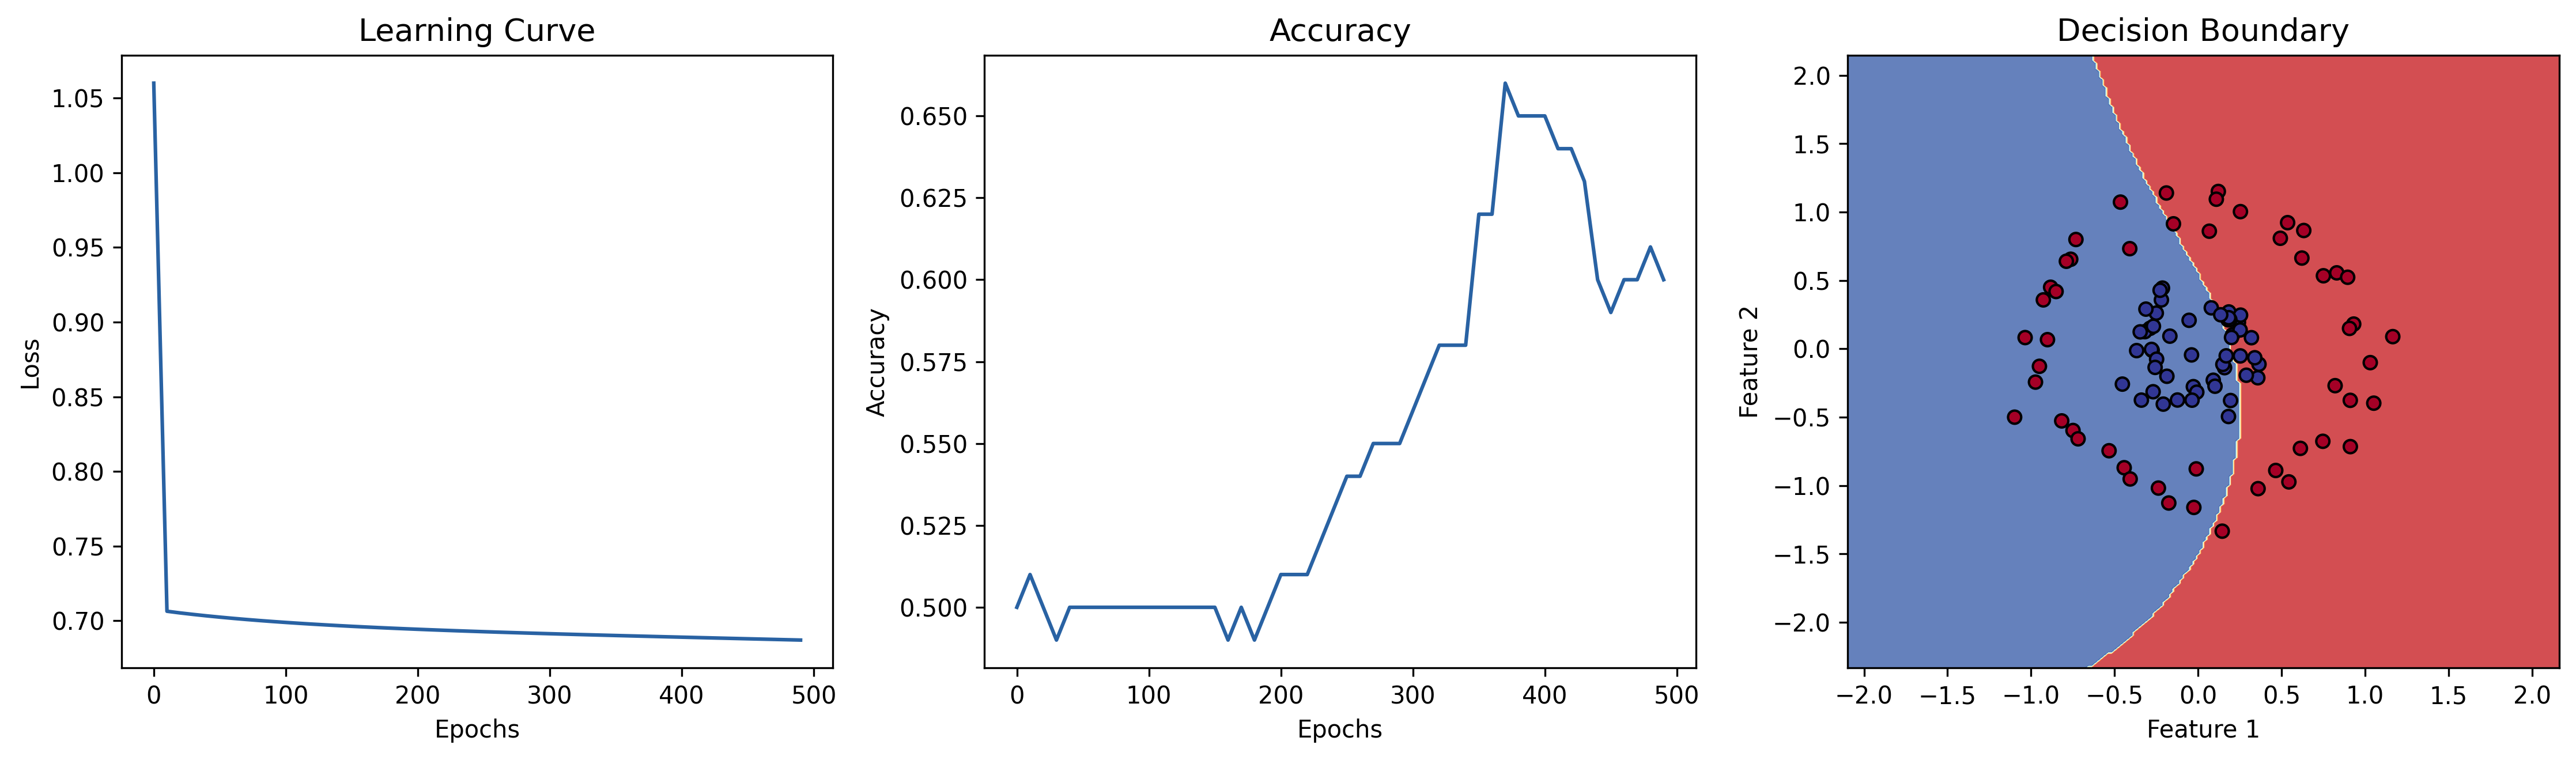
\includegraphics[width=\textwidth]{circles_boundary}
  \caption{Circles dataset --- learning curve, accuracy, and decision boundary. Architecture: \texttt{[2, 32, 32, 1]}, 500 epochs.}
  \label{fig:circles}
\end{figure}

\subsection{Moons --- Still Easy}

\begin{lstlisting}
from sklearn.datasets import make_moons
X, y = make_moons(n_samples=1000, noise=0.15)
X = X.T
y = y.reshape((1, y.shape[0]))

parameters = neural_network(X, y, [2, 64, 64, 1],
                            learning_rate=0.1, epoch=5000)
\end{lstlisting}

The moon-shaped data is harder than circles, but two hidden layers of 64 neurons handle it comfortably. The decision boundary curves smoothly around each crescent.

\begin{figure}[H]
  \centering
  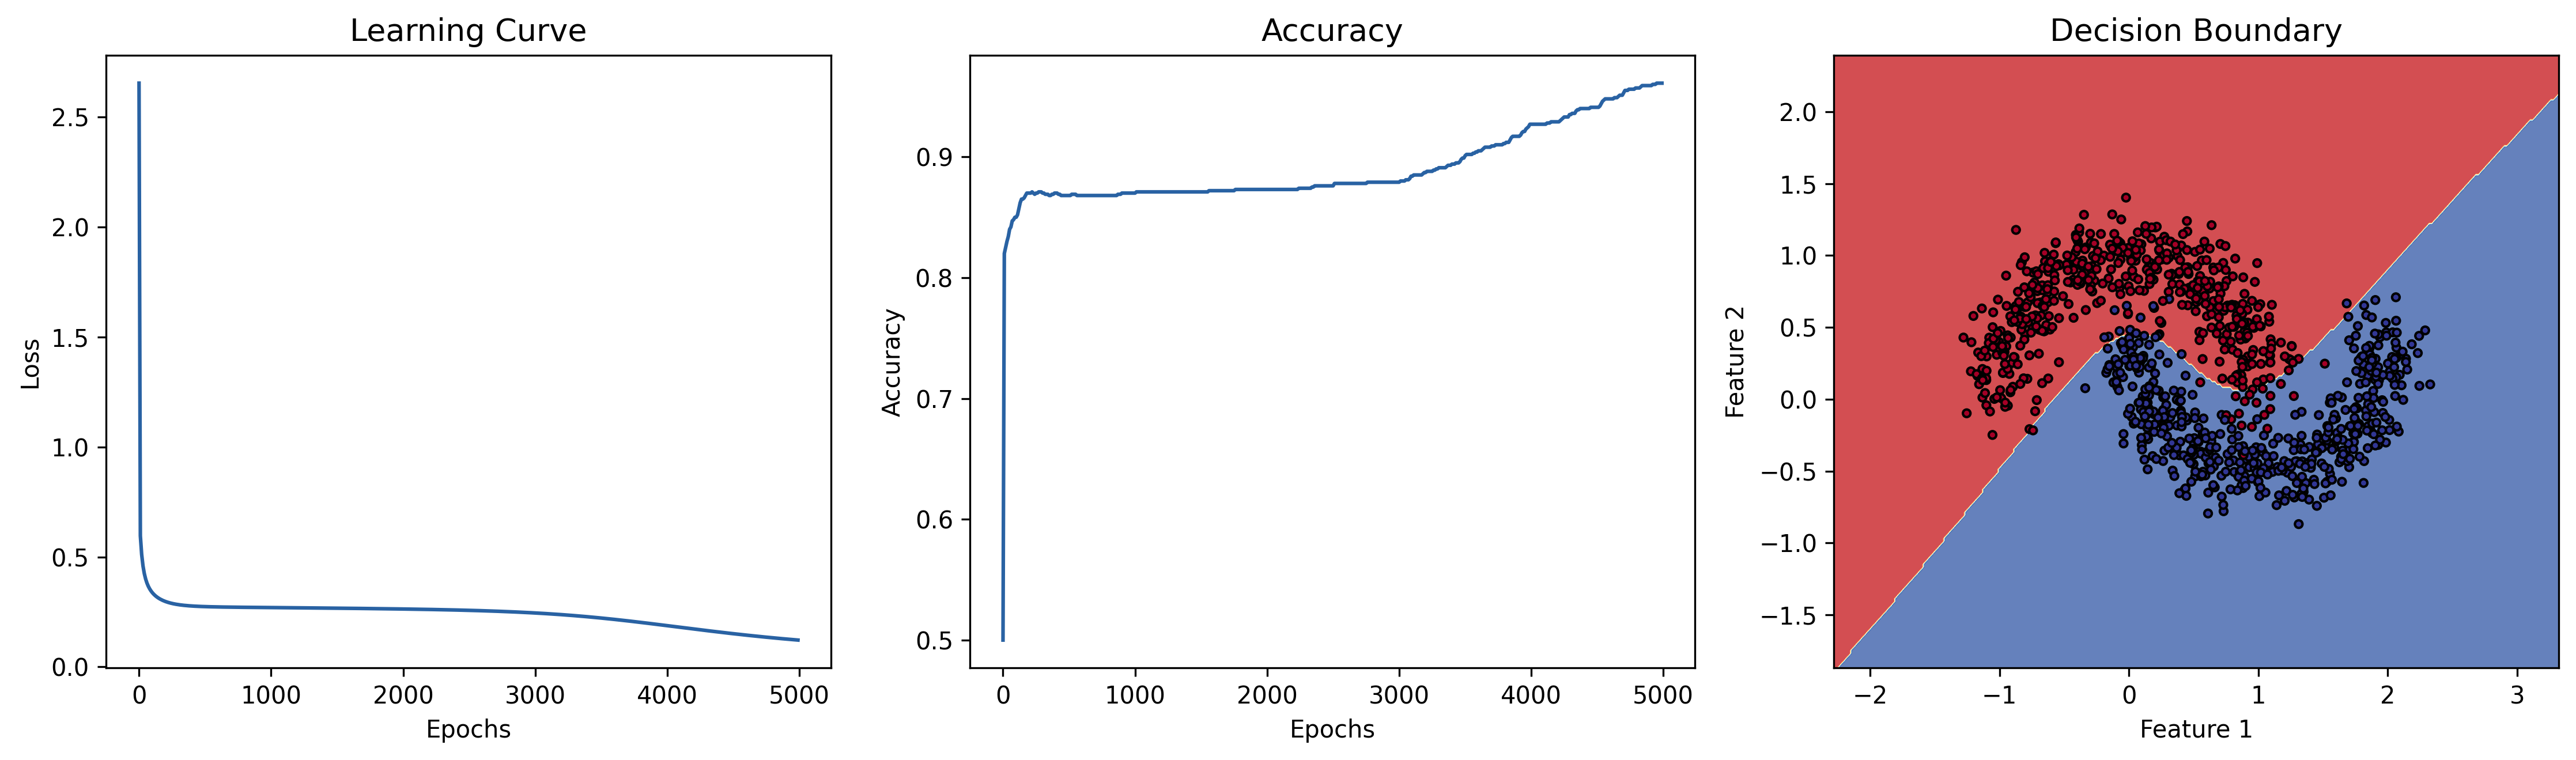
\includegraphics[width=\textwidth]{moons_boundary}
  \caption{Moons dataset --- the network carves a smooth nonlinear boundary between the two crescents. Architecture: \texttt{[2, 64, 64, 1]}, 5000 epochs.}
  \label{fig:moons}
\end{figure}

\subsection{Spirals --- The Real Test}

Now we push the network to its limits:

\begin{lstlisting}
parameters = neural_network(X, y, [2, 64, 64, 64, 1],
                            learning_rate=0.1, epoch=5000)
\end{lstlisting}

\begin{figure}[H]
  \centering
  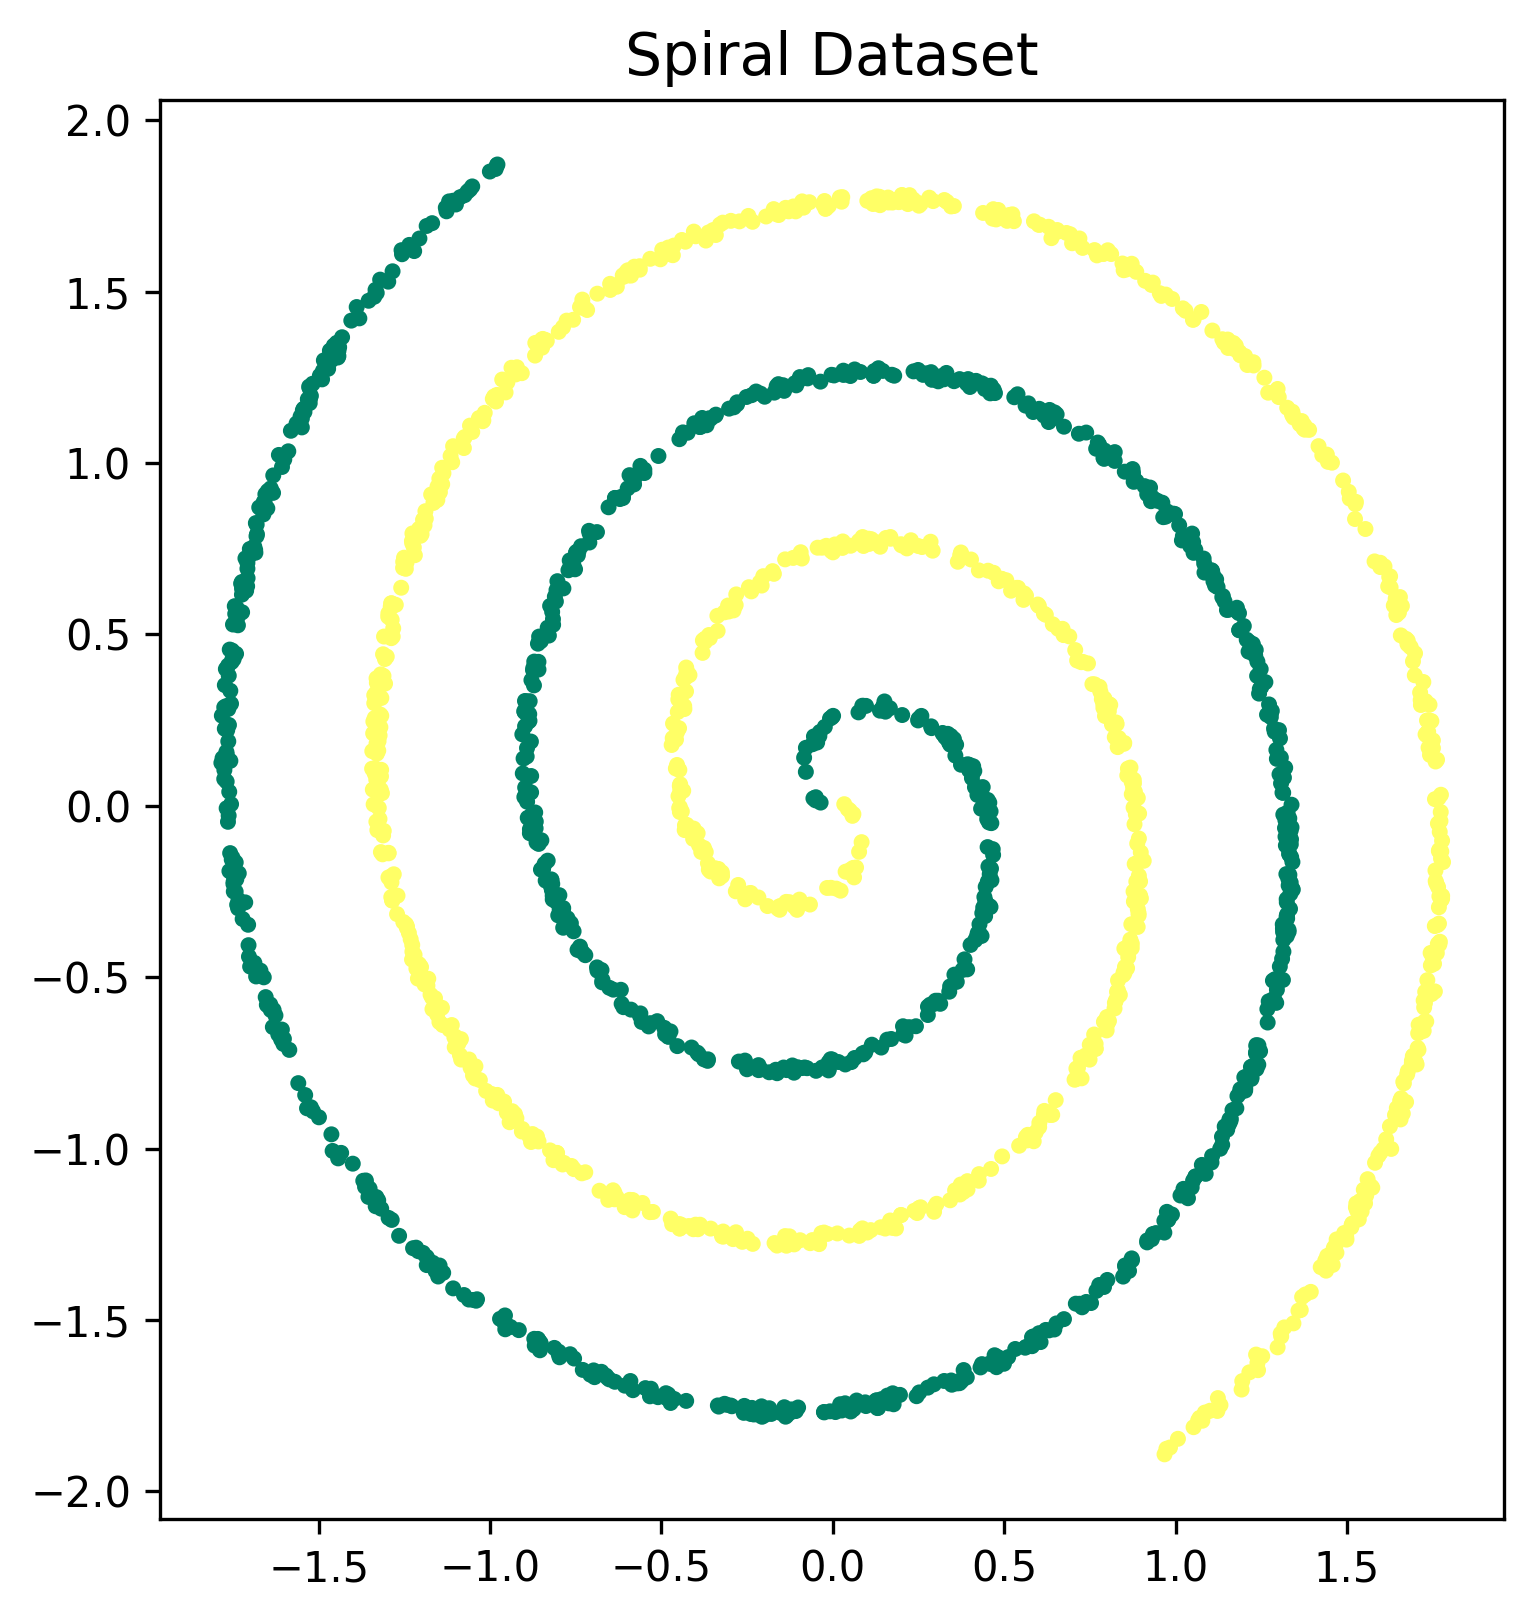
\includegraphics[width=0.45\textwidth]{spirals_data}
  \caption{The spiral dataset --- two interleaved classes wrapping around each other.}
  \label{fig:spirals_data}
\end{figure}

Spirals are interleaved --- the two classes wrap around each other. This is a genuinely hard problem. With three hidden layers, the network reaches around 85\% accuracy. Not perfect, but remember: this is pure NumPy. No frameworks. No tricks.

\begin{figure}[H]
  \centering
  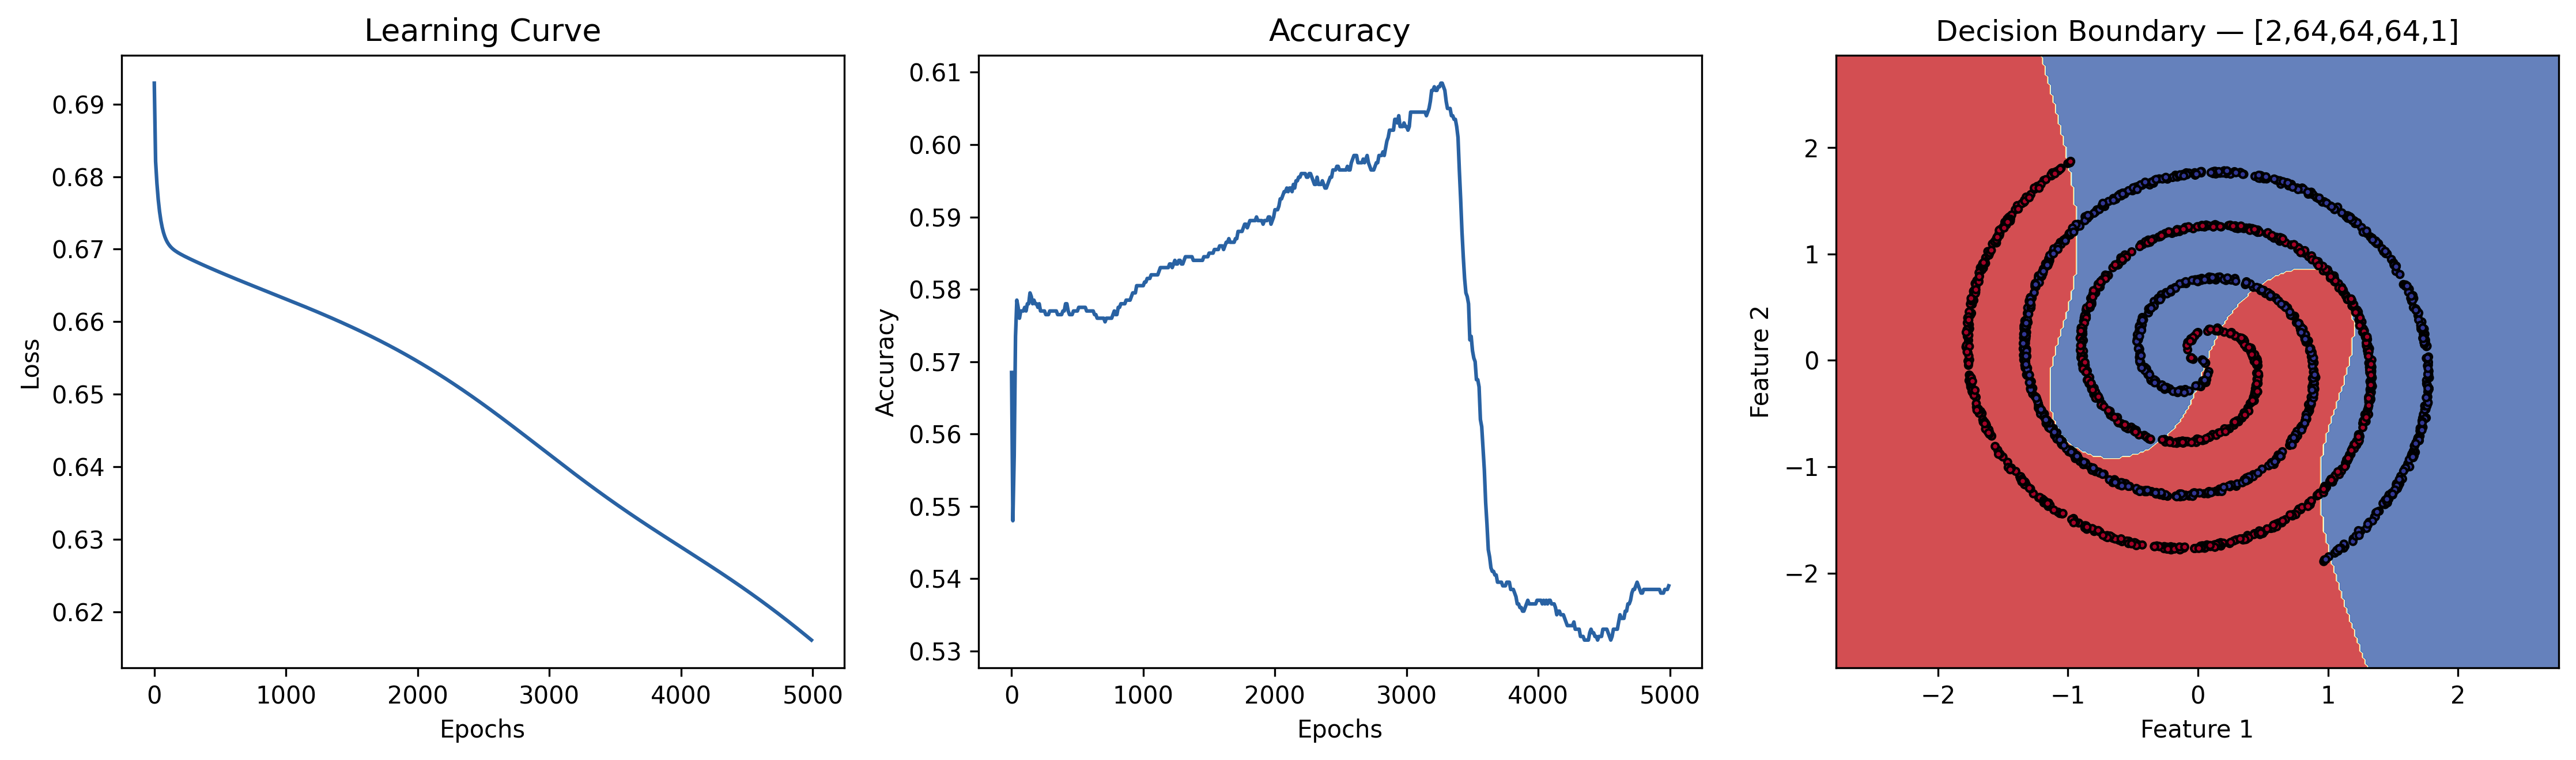
\includegraphics[width=\textwidth]{spirals_boundary}
  \caption{Spirals with 3 hidden layers \texttt{[2, 64, 64, 64, 1]} --- the boundary starts wrapping around the spiral arms.}
  \label{fig:spirals3}
\end{figure}

What if we go deeper?

\begin{lstlisting}
parameters = neural_network(X, y, [2, 128, 128, 128, 128, 1],
                            learning_rate=0.1, epoch=5000)
\end{lstlisting}

Better. More layers, more neurons --- the decision boundary becomes more complex, wrapping tighter around the spiral arms.

\begin{figure}[H]
  \centering
  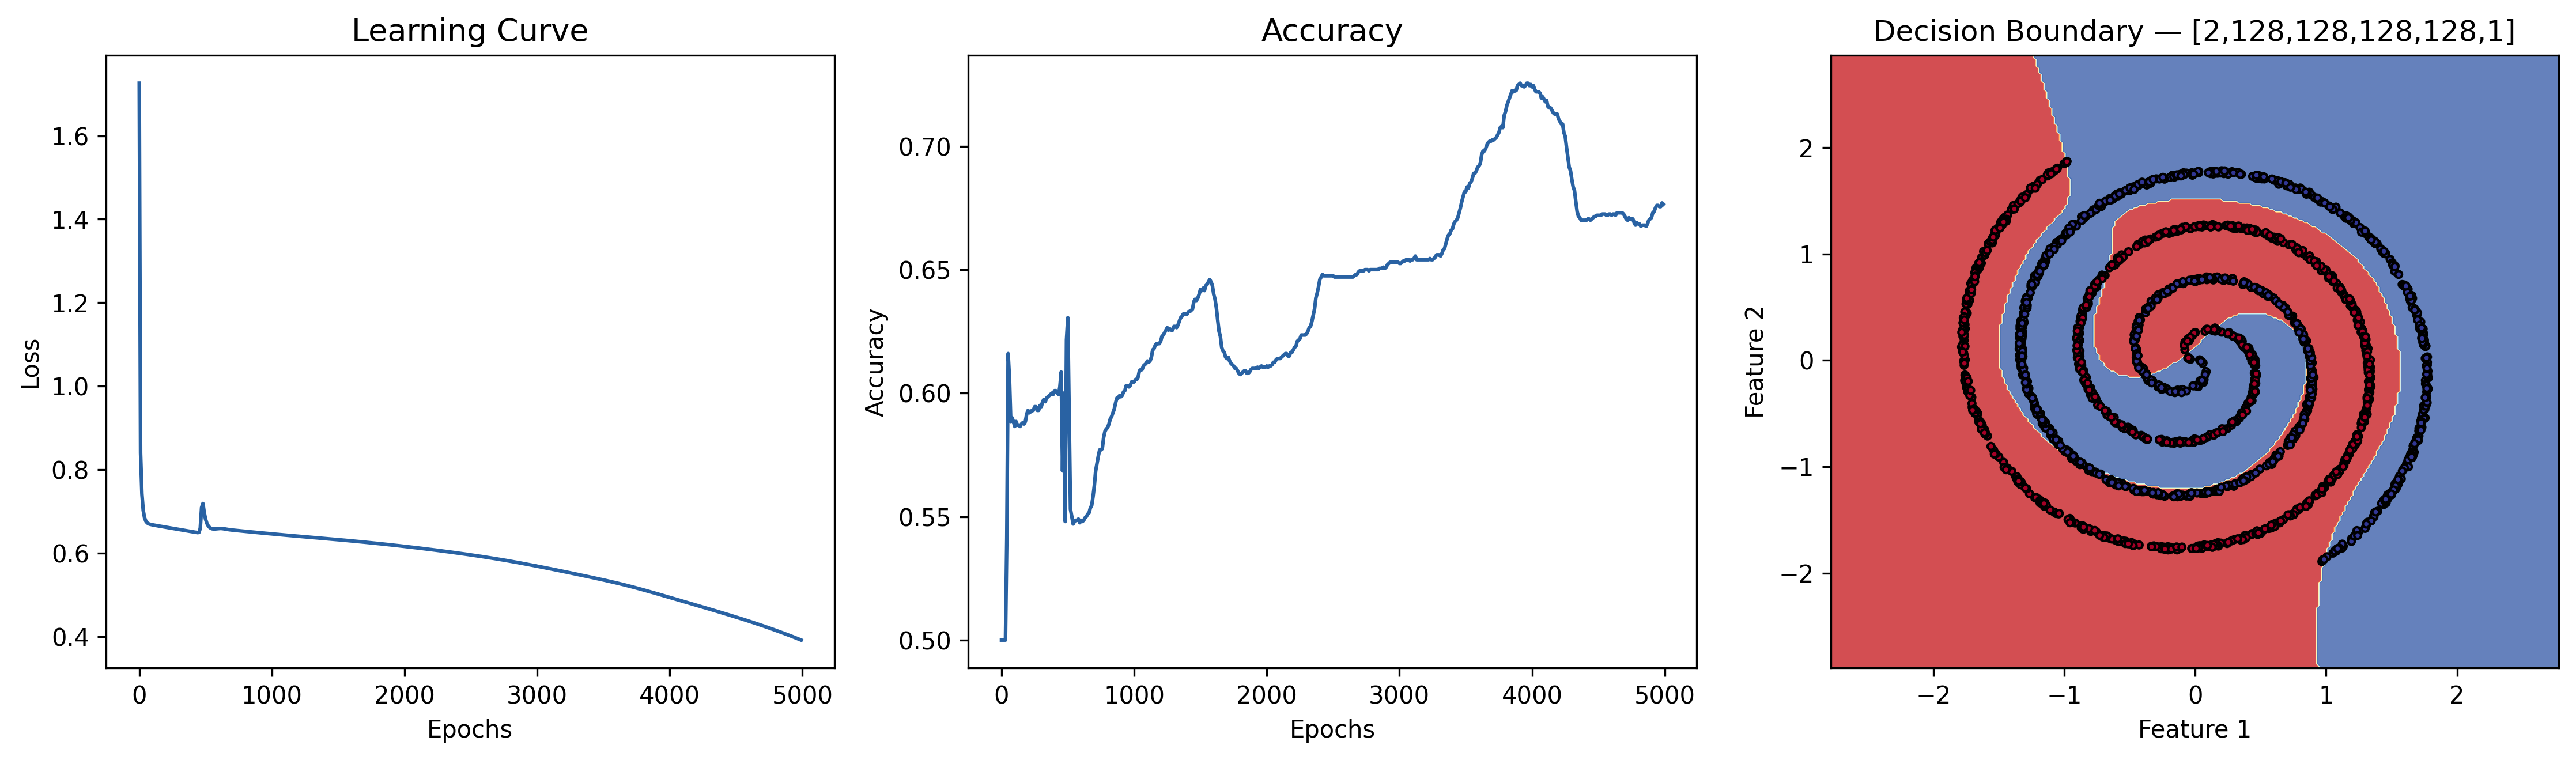
\includegraphics[width=\textwidth]{spirals_deep_boundary}
  \caption{Spirals with 4 hidden layers \texttt{[2, 128, 128, 128, 128, 1]} --- stronger boundary, higher accuracy.}
  \label{fig:spirals4}
\end{figure}

\begin{insightbox}[title=Depth vs Complexity]
More complex data requires \textbf{more layers}. That's the whole point of depth.

\begin{itemize}
  \item \textbf{Circles}: 2 layers suffice (simple nonlinearity)
  \item \textbf{Moons}: 2 layers work, 3 are comfortable
  \item \textbf{Spirals}: 3--4 layers needed (highly nonlinear boundary)
\end{itemize}

Each layer adds another level of \textbf{abstraction} --- the ability to capture more complex patterns.
\end{insightbox}


%% ============================================================
%% SECTION 9 --- REAL DATA
%% ============================================================
\section{Real Data --- Cats vs Dogs, Going Deeper}

Let's go back to the real-world challenge from Episode VI: classifying images of cats and dogs.

The data: $64 \times 64$ pixel images, flattened to 4096-dimensional vectors. 1000 training images, a few hundred for testing.

In Episode VI, we used the equivalent of \texttt{[4096, 32, 32, 1]}. Now we can try deeper architectures. But first, we need a version of the training loop that tracks \textbf{both} training and test performance:

\begin{lstlisting}
def neural_network2(X_train, y_train, X_test, y_test,
                    dimensions, learning_rate, epoch):
    parameters = initialisation(dimensions)
    train_loss, train_acc = [], []
    test_loss, test_acc = [], []

    for i in tqdm(range(epoch)):
        L = len(parameters) // 2
        activations = forward_propagation(X_train, parameters)

        if i % 100 == 0:
            # Training metrics
            train_loss.append(log_loss(y_train.flatten(),
                              activations[f'A{L}'].flatten()))
            predictions = predict(X_train, parameters)
            train_acc.append(accuracy_score(y_train.flatten(),
                             predictions.flatten()))

            # Test metrics
            act_test = forward_propagation(X_test, parameters)
            test_loss.append(log_loss(y_test.flatten(),
                             act_test[f'A{L}'].flatten()))
            pred_test = predict(X_test, parameters)
            test_acc.append(accuracy_score(y_test.flatten(),
                            pred_test.flatten()))

        gradients = back_propagation(y_train, parameters,
                                     activations)
        parameters = update(gradients, parameters, learning_rate)

    # Plot train vs test
    plt.figure(figsize=(12, 4))
    plt.subplot(1, 2, 1)
    plt.plot(train_loss, label='Train Loss')
    plt.plot(test_loss, label='Test Loss')
    plt.legend()
    plt.title('Loss')
    plt.subplot(1, 2, 2)
    plt.plot(train_acc, label='Train Accuracy')
    plt.plot(test_acc, label='Test Accuracy')
    plt.legend()
    plt.title('Accuracy')
    plt.show()

    return parameters
\end{lstlisting}

Now let's try:

\begin{lstlisting}
parameters = neural_network2(
    X_train, y_train, X_test, y_test,
    [X_train.shape[0], 16, 16, 1],
    learning_rate=0.01, epoch=5000
)
\end{lstlisting}

The result will look familiar: training accuracy climbs toward 90--95\%, but test accuracy plateaus around 50--55\%.

\begin{figure}[H]
  \centering
  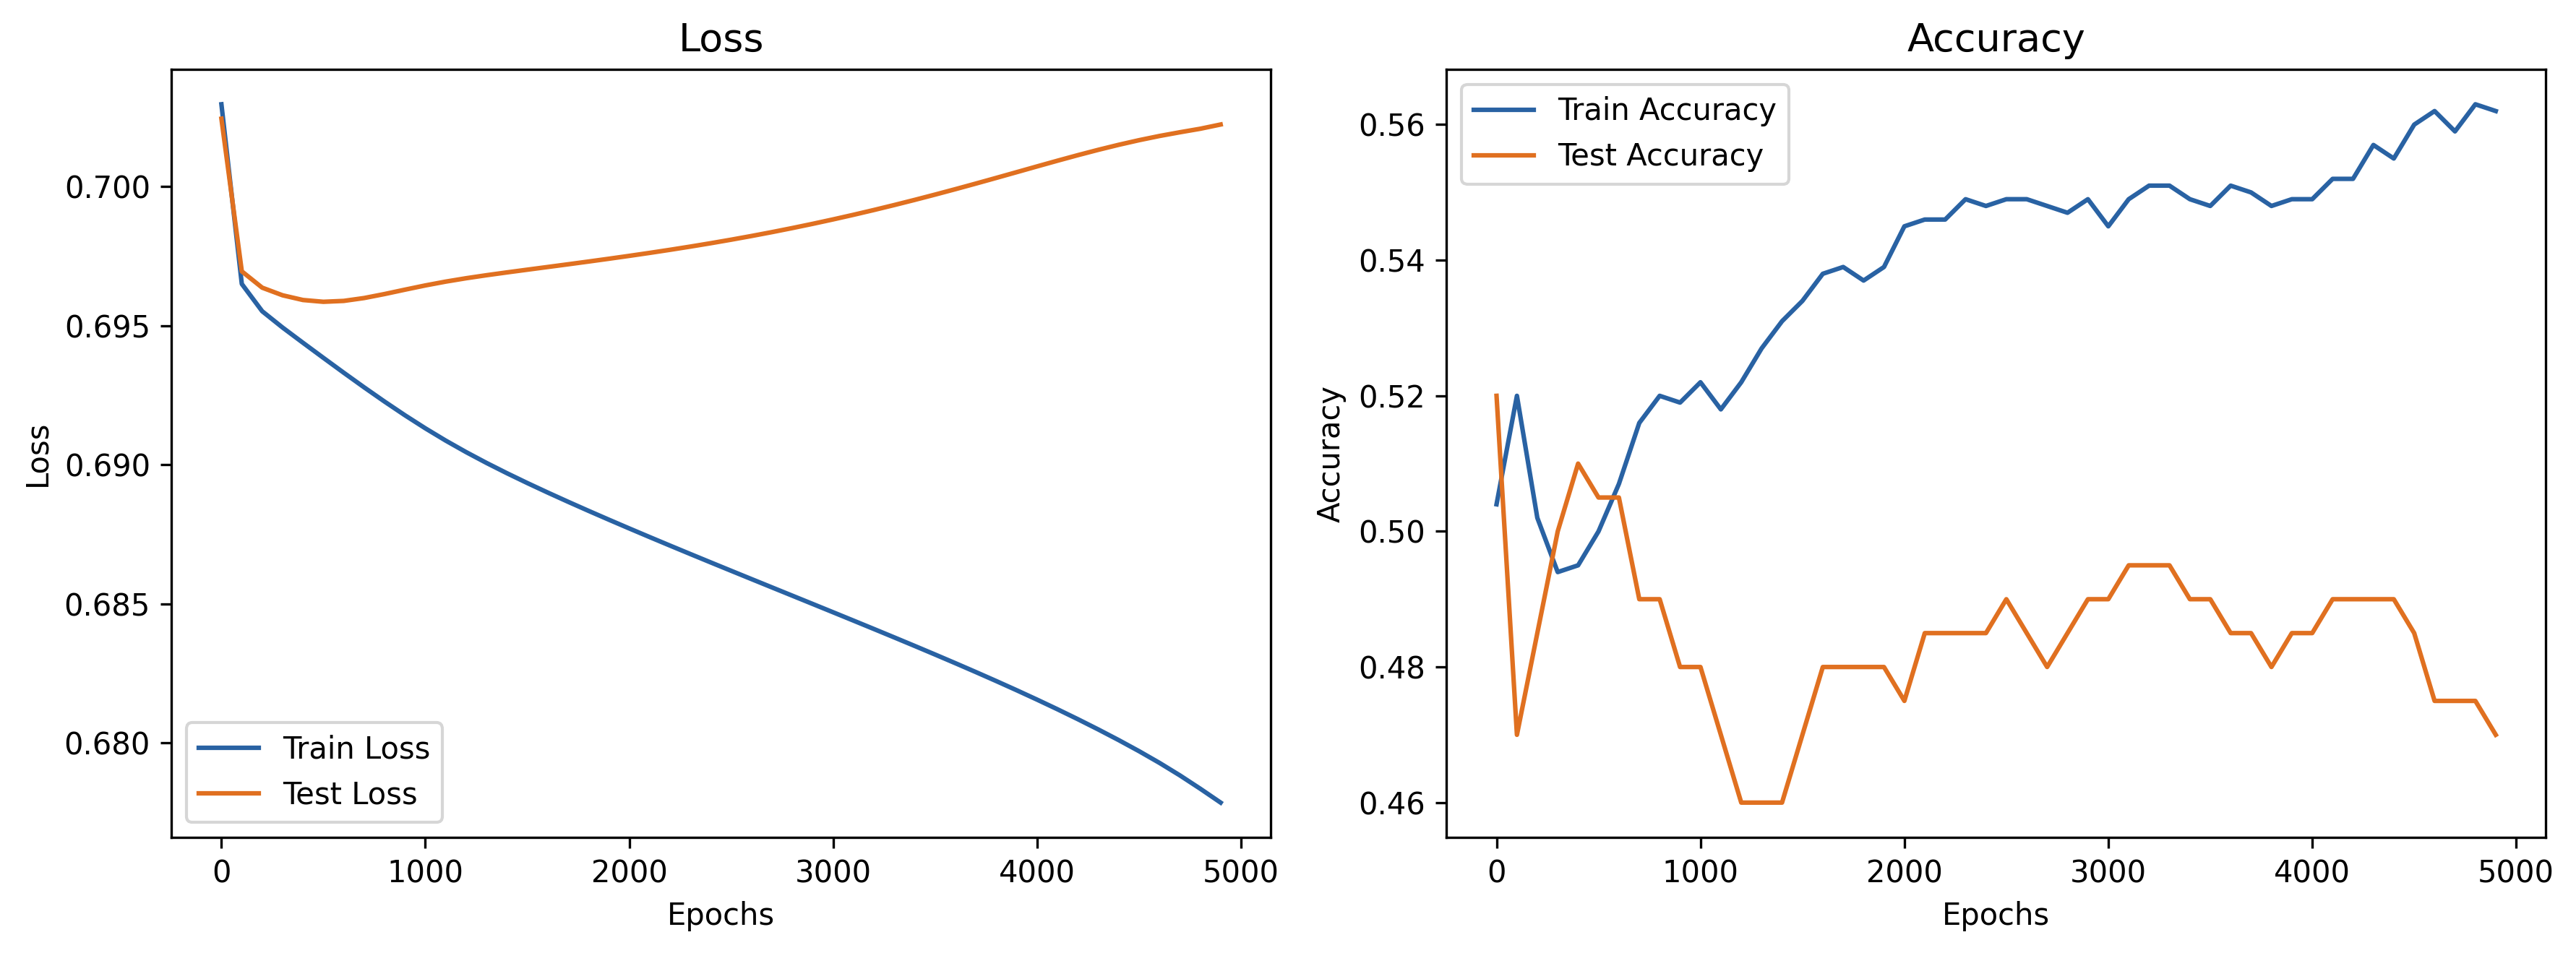
\includegraphics[width=0.9\textwidth]{catsdogs_overfitting}
  \caption{Cats vs dogs --- train loss keeps falling, but test accuracy stays flat. Classic overfitting.}
  \label{fig:catsdogs}
\end{figure}

\textit{The same overfitting wall we hit in Episode VI.}


%% ============================================================
%% SECTION 10 --- THE OVERFITTING WALL
%% ============================================================
\section{The Overfitting Wall}

Here's the uncomfortable truth: adding more layers \textbf{doesn't solve} the overfitting problem.

Try \texttt{[4096, 64, 32, 16, 1]}. Try \texttt{[4096, 128, 64, 32, 16, 1]}. The training accuracy might reach 99\%. But the test accuracy? Still stuck around 50--55\%.

\begin{warnbox}[title={More Depth $\neq$ Better Generalization}]
More layers give the network more \textbf{capacity} --- the ability to learn more complex patterns. But capacity without discipline is dangerous.

A deeper network can memorize the training data more efficiently. It doesn't mean it \textbf{understands} the data.
\end{warnbox}

This is the same lesson from Episode VI, but now it's even more striking. We can build a network of \textit{any depth}, and it still can't break the 55\% barrier on test data.

Why?

\begin{enumerate}
  \item \textbf{Not enough data.} 1000 images isn't enough to train a network with thousands of parameters.
  \item \textbf{No regularization.} We have no mechanism to prevent the network from overfitting.
  \item \textbf{Optimization challenges.} Deep networks with sigmoid activations can suffer from vanishing gradients --- the error signal becomes too small to update the early layers effectively.
\end{enumerate}

\begin{insightbox}[title=The Million-Dollar Question]
When your model fails, always ask:

\begin{quote}
\textbf{``Is this a problem with the data, the model, or the training?''}
\end{quote}

Here, it's \textbf{all three}:
\begin{itemize}
  \item \textbf{Data}: not enough images for this task
  \item \textbf{Model}: sigmoid activation causes vanishing gradients in deep networks
  \item \textbf{Training}: no regularization, no dropout, no data augmentation
\end{itemize}

Each of these has a solution. But that's the next chapter.
\end{insightbox}


%% ============================================================
%% SECTION 11 --- WHAT YOUVE BUILT
%% ============================================================
\section{What You've Built}

Take a step back and look at what just happened.

In Episode VI, you coded a neural network with two layers. Today, you \textbf{removed the constraint}. You generalized five functions --- and now you can build a network of \textbf{any depth}.

\begin{resultbox}[title=Your Deep Neural Network --- From Scratch]
\begin{enumerate}[label=\textbf{\arabic*.}]
  \item \textbf{Architecture definition}: a single \texttt{dimensions} list
  \item \textbf{Initialization}: one loop creates all $W_l$ and $b_l$
  \item \textbf{Forward propagation}: one loop computes all $A_l$
  \item \textbf{Backpropagation}: one backward loop computes all gradients
  \item \textbf{Update}: one loop applies gradient descent to all parameters
  \item \textbf{Training loop}: identical structure, works for any depth
  \item \textbf{Testing}: circles, moons, spirals, cats vs dogs
\end{enumerate}
\end{resultbox}

The code for a 2-layer network and a 100-layer network is \textbf{the same}. Only the dimensions list changes.

That's the power of generalization.

\begin{quote}
\textit{You don't need a bigger codebase. You need a smarter one.}
\end{quote}

\section{What's Next}

You now have the power to build deep networks. But power without discipline leads to overfitting, vanishing gradients, and wasted computation.

The next step isn't more layers. It's learning how to \textbf{control} what we've built.

\begin{actionbox}[title=Next Stop --- Discipline]
We need to teach the network discipline:
\begin{itemize}
  \item \textbf{Better activations}: ReLU instead of sigmoid
  \item \textbf{Regularization}: preventing memorization
  \item \textbf{Better optimization}: beyond basic gradient descent
  \item \textbf{More data}: or smarter use of what we have
\end{itemize}

Depth is the foundation. Discipline is what makes it work.

\textbf{Meet me in the next episode.}
\end{actionbox}

\vspace{2em}
\begin{center}
\rule{0.6\textwidth}{0.4pt}\\[1em]
{\small \textbf{Deep Learning From Scratch}}\\[0.3em]
{\small An open-source learning journey.}\\[0.8em]
{\small \textbf{GitHub:} \url{https://github.com/Pchambet/Deep-Learning-from-Scratch}}\\[0.3em]
{\small \textbf{LinkedIn:} \url{https://www.linkedin.com/in/pierre-chambet/}}\\[1em]
{\footnotesize \textcopyright\ 2026 Pierre Chambet}
\end{center}

\end{document}
